\documentclass{beamer}

%\colorlet{structure}{red!65!black}
%
%\beamertemplateshadingbackground{blue!40}{white}
%
\usepackage{beamerthemesplit}
%\usepackage{hyperref}
\usetheme{Berkeley}
\useinnertheme{circles}
\usecolortheme{seagull}

\title[Stereo vision]{Stereo Vision using the OpenCV library \\ Halfway report}
\author[Dr\"oppelmann \and Hueting \and Latour \and \\Van der Veen]{Sebastian Dr\"oppelmann \\ Moos Hueting \\ Sander Latour \\ Martijn van der Veen}
\institute{University of Amsterdam}
\date{June 2010}
\subject{Computer vision}

\begin{document}

\graphicspath{{./images/}}

\frame
{
  \titlepage
}

\section{Recap}

\frame
{
 \frametitle{Goal}
 \begin{block}{Goal}
   Generating a disparity depth map of the environment using stereo vision.
 \end{block}
}

\frame{
 \frametitle{Intended end-result}
 \begin{figure}
   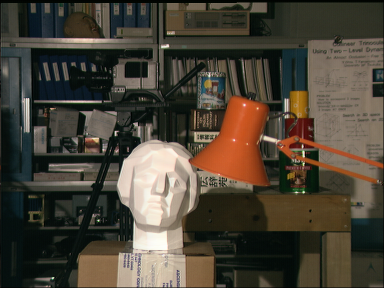
\includegraphics[width=0.3\textwidth]{exampleleft}
   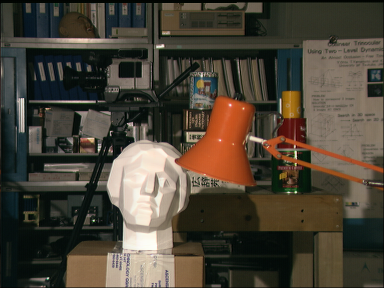
\includegraphics[width=0.3\textwidth]{exampleright}
   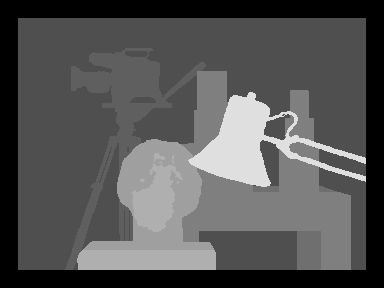
\includegraphics[width=0.3\textwidth]{exampledepth}
   \caption{Stereo images with disparity depth map}
 \end{figure}
}


\section{Results}

\frame{
 \frametitle{Stereo calibration}
 \begin{itemize}
   \item Estimating transformation between stereo camera pair
   \item Use chessboards
   \begin{itemize}
     \item Demo
   \end{itemize}
   \item Practical problems
\end{itemize}
}

\frame{
  \frametitle{Stereo rectification}
  \begin{itemize}
    \item Transform to make epipolar lines...
    \begin{itemize}
      \item ...horizontal
      \item ...colinear
    \end{itemize}
  \end{itemize}
}

\frame{
  \frametitle{Unrectified images}
  \begin{figure}
    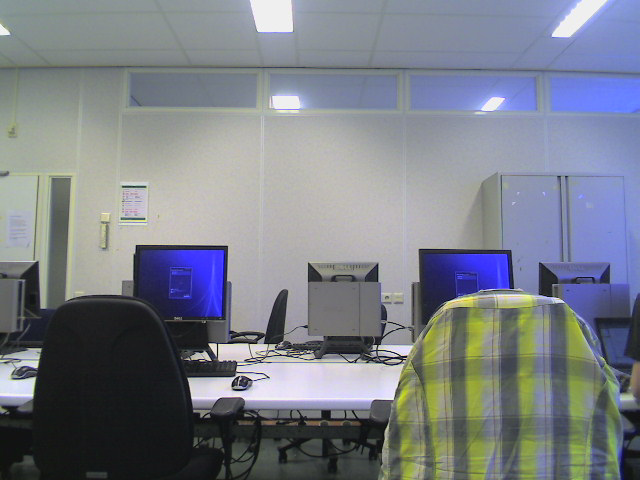
\includegraphics[width=0.5\textwidth]{leftown}
    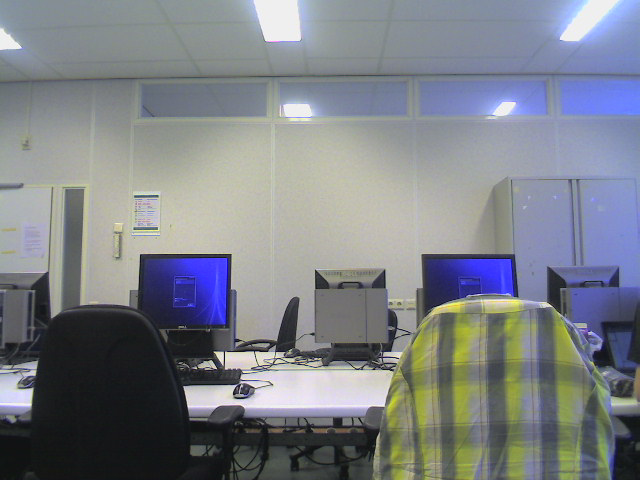
\includegraphics[width=0.5\textwidth]{rightown}
  \end{figure}
}

\frame{
  \frametitle{Rectified images}
  \begin{figure}
    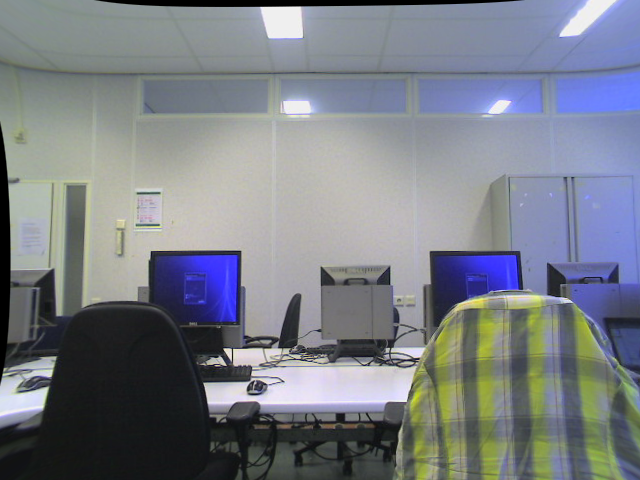
\includegraphics[width=0.5\textwidth]{leftownr}
    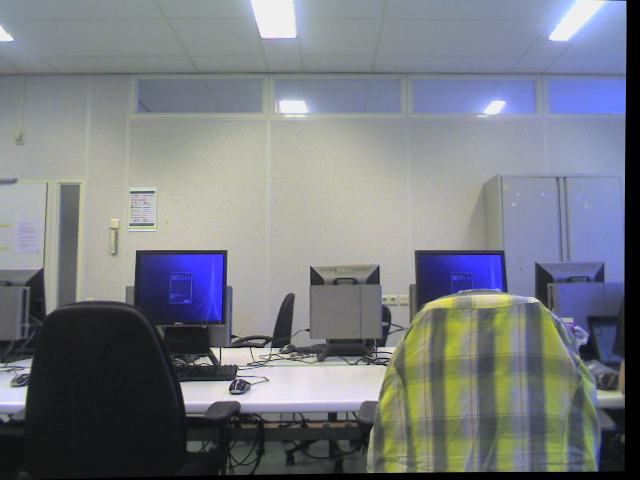
\includegraphics[width=0.5\textwidth]{rightownr}
  \end{figure}
}

\section{Depth Map Algorithms}


\frame
{
  \frametitle{Depth Map Algorithms}
  
  Tested with standard OpenCV algorithms\\
  Used datasets from Middlebury\\

  \begin{itemize}
    \item Graph Cut
    \item Block Matching
    \item Semi Global Block Matching
  \end{itemize}
  
}

\frame {
  \frametitle{New Problems}
  \begin{itemize}
    \item parameters of algorithms
    \item understand and choose right occlusion handling
    \item implementation very bad with twisted cameras
  \end{itemize}
}

\frame {
  \frametitle{Graph Cut}
      \begin{itemize}
      \item popular
      \item slow
      \item good noise detection
      \end{itemize}
      \begin{figure}
      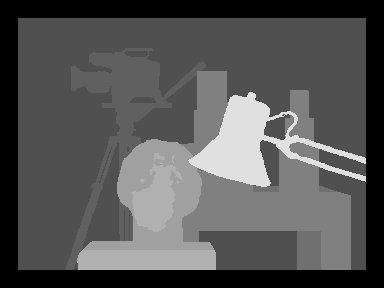
\includegraphics[width=0.4\textwidth]{disp_tsukuba_orig}
      \:
      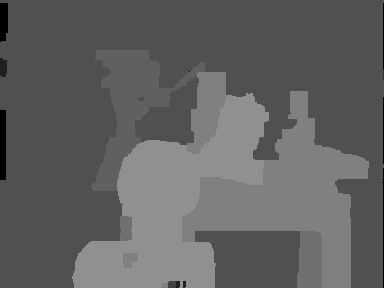
\includegraphics[width=0.4\textwidth]{gc_tsukuba_own}
      \end{figure}
}


\frame {
  \frametitle{Block Matching}
    \begin{itemize}
      \item faster
      \item interpretation missing
    \end{itemize}
    \begin{figure}
    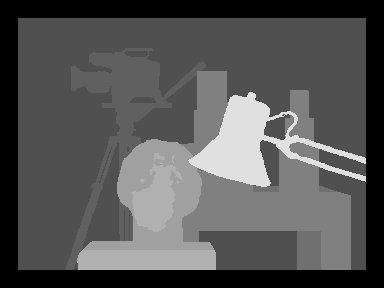
\includegraphics[width=0.4\textwidth]{disp_tsukuba_orig}
    \:
    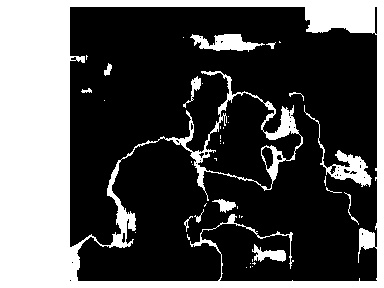
\includegraphics[width=0.4\textwidth]{bm_tsukuba_own}
    \end{figure}

}

\frame{
    \frametitle{Semi Global Block Matching}
    \begin{itemize}
      \item not in Python (used C++ implementation)
      \item fastest
      \item good depthmap
      \item much noise (needs tuning)
    \end{itemize}
    \begin{figure}
    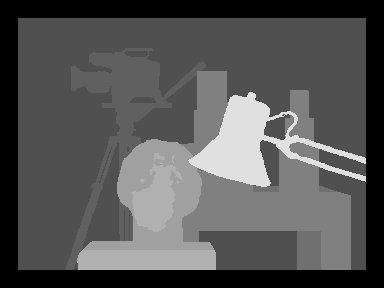
\includegraphics[width=0.4\textwidth]{disp_tsukuba_orig}
    \:
    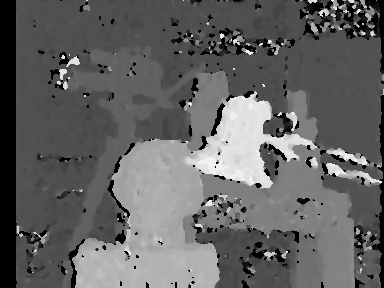
\includegraphics[width=0.4\textwidth]{sgbm_tsukuba_own}
    \end{figure}
}



\section{Planning}
\frame
{
  \frametitle{Planning}
  \begin{itemize}
    \item Week 1
      \begin{itemize}
        \item {\bf done} Reading literature
        \item {\bf done} Getting webcams to work
        \item {\bf done} Choosing dense algorithm
      \end{itemize}
    \item Week 2 and 3
      \begin{itemize}
        \item Implementing
          \begin{itemize}
            \item \emph{done} Camera calibration
            \item {\bf done} Rectification of images using epipolar geometry
            \item \emph{done} Dense disparity map algorithm
          \end{itemize}
        \item Halfway report
      \end{itemize}
    \item Week 4
      \begin{itemize}
        \item Optimizing and testing
        \item If there's enough time left
          \begin{itemize}
            \item Generate 3D image of environment
            \item Remove background using dense disparity map
          \end{itemize}
      \end{itemize}
  \end{itemize}
}

\frame {
  \frametitle{New planning - week 3}
  \begin{itemize}
    \item Martijn and Moos
    \begin{itemize}
      \item Fine tuning calibration
      \item Cropping of rectified images
    \end{itemize}
    \item Sebastian and Sander
    \begin{itemize}
      \item Fine tuning parameters
      \item Completely understand the algorithms
      \item Depth map normalize
    \end{itemize}
  \end{itemize}
}
\end{document}
